\section{Preliminaries}\label{sec:preliminaries}

The network consists of two
node types: \emph{Full nodes} are responsible for
verifying the chain and mining new blocks. \emph{Verifiers} connect to full nodes to learn facts
about the chain without downloading it, such as whether a
transaction is confirmed. A verifier connects to multiple full nodes, which function as \emph{provers} for the verifier, at
least one of which is honest.
We model full nodes according to Backbone~\cite{backbone}. There are
$n$ full nodes, of which $t$ are adversarial and $n - t$ honest. All $t$
parties are controlled by one colluding adversary $\mathcal{A}$.
%The
%parties have access to a hash function $H$ modelled as a common Random
%Oracle~\cite{ro}. To each novel query, the random oracle outputs $\kappa$ bits
%of fresh randomness. Time is split into distinct \emph{rounds} numbered by the
%integers $1, 2, \cdots$. Our treatment is in the \emph{synchronous model}, so we
%assume messages \emph{diffused} (broadcast) by an honest party at the end of a
%round are received by all honest parties at the beginning of the next round.
%This is equivalent to a network connectivity assumption in which the round
%duration is taken to be the known time needed for a message to cross the
%diameter of the network. The adversary can inject messages, reorder them, sybil
%attack~\cite{sybil} by creating multiple messages, but not suppress messages.

Each honest full node locally maintains a \emph{chain} $\chain$, a sequence of
blocks. From now on we will
use the term \emph{block} to mean
\emph{block header}. Each block contains a Merkle Tree root~\cite{merkle} of
transaction data
%\footnote{The compression of
%$\overline{x}$ is beyond the scope of our work. Vendors verifying a small number
%of transactions benefit exponentially from a superlight client even without
%compressing $\overline{x}$.}
$\overline{x}$, the hash $s$ of the previous block in the chain
(\emph{previd}), and a nonce $ctr$. Each block $b = s \conc
\overline{x} \conc ctr$ satisfies the PoW~\cite{pow} equation $H(b) \leq T$
where $T$ is a constant \emph{target}, a small value signifying the difficulty. We assume $T$ is constant\footnote{Variable difficulty NIPoPoWs have been explored in the soft fork
case~\cite{dionyziz}. We leave the treatment of velvet NIPoPoWs in
variable difficulty for future work.}. $H(b)$ is
known as the \emph{block id}.

Blockchains are finite block sequences obeying the \emph{blockchain property}:
every block in the chain contains a pointer to its previous one. A
full valid chain begins with the \emph{genesis} block $\mathcal{G}$,
a special block known to all. The verifier only knows about $\mathcal{G}$
when it boots. For chain addressing we use Python brackets $\chain[\cdot]$. A
zero-based positive index indicates the indexed block.
A negative index indicates a block from the end, e.g., $\chain[-1]$ is
the \emph{tip}. A range $\chain[i{:}j]$ is a subarray from
$i$ (inclusive) to $j$ (exclusive). Given chains $\chain_1, \chain_2$ and blocks
$A, Z$ we concatenate them as $\chain_1 \chain_2$ or $\chain_1 A$ (we also use $\conc$ for concatenation). Here,
$\chain_2[0]$ must point to $\chain_1[-1]$ and $A$ must point to $\chain_1[-1]$.
We denote $\chain\{A{:}Z\}$ the subarray from block $A$ (inclusive) to
block $Z$ (exclusive). We omit blocks or indices from either side of the range to
take the chain to the beginning or end respectively. If the blockchain
property is maintained, we use set operators $\cup$, $\cap$ and
$\subseteq$ between chains, implying that
blocks are selected and then ordered chronologically.

At every round, every honest party attempts to \emph{mine} a block on top of
its chain. Each party is given $q$ queries to the random
oracle to mine. The adversary
has $tq$ queries per round while each honest party has $(n - t)q$ queries per
round. When an honest party discovers a new block, they extend their chain
and broadcast it. Upon receiving a chain $\chain'$ from the
network, an honest party compares its length $|\chain'|$ against its currently
adopted length $|\chain|$ and adopts the new chain if longer.
The \emph{honest majority assumption} states that
honest parties control the majority of compute power:
$t < (1 -  \delta)(n - t)$ for some $0 < \delta < 1$. The protocol
ensures consensus: There is a $k$, the
\emph{Common Prefix} parameter, such that, at any round, chains
belonging to honest parties share a common prefix; the chains
differ only up to $k$ blocks at the end~\cite{backbone}.

Some valid blocks satisfy the PoW equation better than required. If
block $b$ satisfies $H(b) \leq 2^{-\mu} T$ for some
$\mu \in \mathbb{N}$ we say that $b$ is a \emph{$\mu$-superblock} or a block
\emph{of level} $\mu$. The probability of a new valid block achieving level
$\mu$ is $2^{-\mu}$. The number of levels in the chain is $\log|\chain|$
with high probability~\cite{popow}. Given chain $\chain$, we denote
$\chain\upchain^\mu$ the subset of $\mu$-superblocks of $\chain$.

\emph{NIPoPoW} protocols allow verifiers to
learn the most recent $k$ blocks of the chain adopted by an honest full
node. The challenge lies in building a
verifier who can find the suffix of the longest chain between claims of both
honest and adversarial provers, while not downloading all block headers. Towards
that goal, the \emph{superblock} approach uses superblocks as PoW samples.
The prover sends superblocks to the verifier to convince them
that PoW has taken place without actually presenting all this
work. The protocol is parametrized by a security parameter
$m$. It determines how many superblocks the prover will send to the verifier.
The prover selects various levels $\mu$ and for each such level sends a
carefully chosen portion of its $\mu$-level \emph{superchain}
$\chain\upchain^\mu$ to the verifier. In protocols such as
Bitcoin and Ethereum, each block $\chain[i + 1]$ points to its
previous block $\chain[i]$, but each $\mu$-superblock $\chain\upchain^\mu[i +
1]$ does not point to its previous $\mu$-superblock $\chain\upchain^\mu[i]$.
An adversarial prover should not be able to reorder the blocks within a
superchain. To allow the verifier to check this, each $\mu$-superblock
points to its most recent preceding $\mu$-superblock. The proposal is
therefore to \emph{interlink} the chain by having each $\mu$-superblock include
a pointer to its most recently preceding $\mu$-superblock. To ensure
integrity, this pointer must be included in the block header and verified by
PoW. However, the miner does not know which level a candidate block
will attain prior to mining it. Therefore, each block is proposed to
include a pointer to the most recently preceding $\mu$-superblock, for every
$\mu$, as illustrated in Figure~\ref{fig.hierarchy}. This only adds
$\log|\chain|$ pointers to each block header.

\begin{figure}[ht]
    \centering
    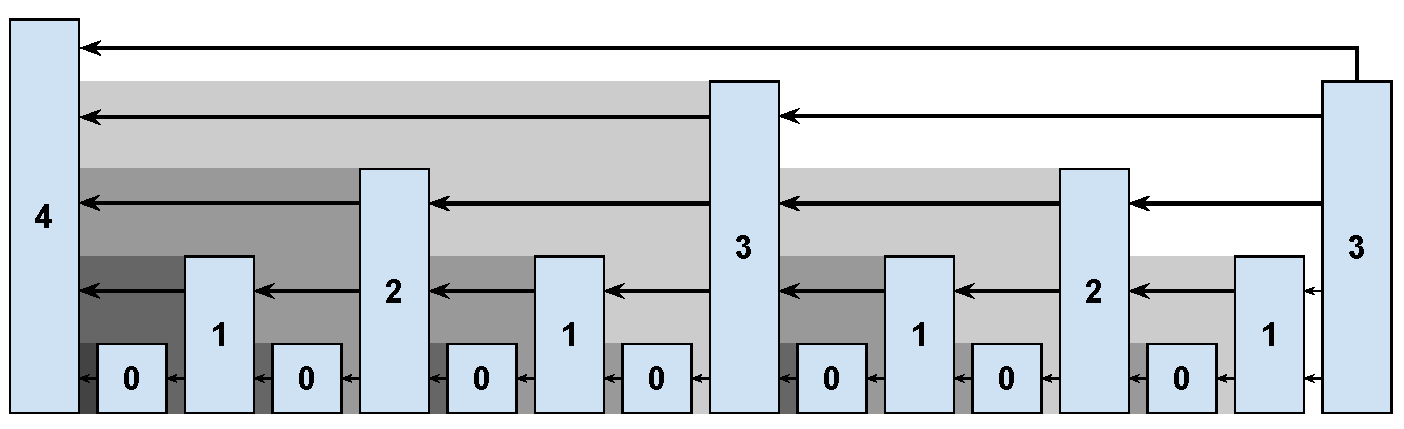
\includegraphics[width=0.8\columnwidth,keepaspectratio]{figures/level-shadows.pdf}
    \caption{An interlinked chain. Each superblock is drawn taller
    according to its level. A block links to all blocks that are
    not overshadowed by descendants. The most recent (right-most)
    block links to the four blocks it has direct line-of-sight to.}
    \label{fig.hierarchy}
\end{figure}

The NIPoPoW protocol can be in short described like this: The prover holds a full chain
$\chain$. When the verifier requests a proof, the prover sends the last $k$
blocks of their chain, the suffix $\chi = \chain[-k{:}]$, in full. From the
prefix $\chain[{:}{-k}]$, the prover constructs a proof $\pi$ by selecting
certain superblocks as representative samples of the PoW.
For each superblock level he adds at least $m$ superblocks.

Upon receiving two proofs $\pi_1\chi_1, \pi_2\chi_2$ of this form, the verifier
first checks that $\lvert \chi_1 \rvert = \lvert \chi_2 \rvert = k$ and that
$\pi_1 \chi_1$ and $\pi_2 \chi_2$ form valid chains. To check this, he
ensures every block in the
proof contains a pointer to its previous block in the proof through either
\emph{previd} or an interlink pointer. It then
compares $\pi_1$ against $\pi_2$ as follows: for each proof, he chooses the superblock level containing the most PoW in comparison to all other levels in the proof. Finally, he compares these two selected superblock levels in terms of the aggregate PoW included and the one with more PoW is accepted. For a detailed description, see Appendix~\ref{sec:nipopows_protocol}.

Blockchains can be upgraded using hard or soft
forks~\cite{buterinforks}. In a \emph{hard fork}, blocks produced by
upgraded miners are not accepted by unupgraded miners. It is simplest to
introduce interlinks using a hard fork mandating that interlink pointers are
included in the header.
To ensure the header is of constant size, instead of including all these
superblock pointers in the header individually, they are organized into a
Merkle Tree of interlink pointers and only the root is
included in the header. In this case, the prover wishing to
show a block $b$ in their proof is connected to its more recently preceding
$\mu$-superblock $b'$ also includes a Merkle Tree proof proving $H(b')$ is
a leaf in the interlink Merkle Tree included in the header of $b$.
The verifier verifies these Merkle proofs.

In a \emph{soft fork}, blocks created by unupgraded miners are not accepted by
upgraded miners, but blocks created by upgraded miners are accepted by
unupgraded miners. Additional data introduced by the upgrade is
included in a field treated as a comment by unupgraded miners.
To soft fork interlink the chain, the interlink Merkle Tree root is
placed in the \emph{coinbase} transaction. Upgraded
miners include the correct interlink tree root in their coinbase and validate
the tree root of blocks.
Unupgraded miners ignore this data and accept the block
regardless.
When a prover wishes to show that a
block $b$ in the proof contains a pointer to its most recently preceding
$\mu$-superblock $b'$, it accompanies the header of $b = s \conc
\overline{x} \conc ctr$ with the coinbase transaction $\coinbase$ of $b$ and
two Merkle Tree proofs: One proving $\coinbase$
is in $\overline{x}$, and one proving $H(b')$ is in the interlink
Merkle Tree whose root is in $\coinbase$.
